% !TEX root =  paper.tex

\section{Evaluation}
\label{sec:evaluation}

To evaluate our proposed technique,
we design a study aiming at answering
the following research questions:

\begin{enumerate}[label=\textbf{RQ\arabic*}, leftmargin=*]
	\item What is the accuracy of \toolName in identifying actionables?
	\item Does \toolName improve the
	exploration of web apps in terms of coverage?
\end{enumerate}



\subsection{RQ1: Accuracy of the actionable prediction models}

\subsubsection{Study design}
As mentioned,
we randomly choose 20\% of the websites 
from our initial dataset
for our testing set,
which includes 139,521 elements,
out of which 74,129 are actionable
(incorporating the event propagation).
We report the accuracy of the trained models
using the following measures commonly used in
evaluating the performance of machine learning models:

\header{Precision} The \textit{precision} of a classification model
for a class $c$
is defined as the ratio of the instances that the model correctly classifies 
to belong to the class $c$
(i.e., true positives)
compared to all the instances that the model classifies (correctly and incorrectly) to belong to $c$.
The precision is therefore calculated as
$\text{Precision}_{c} = \frac{TP_{c}}{TP_{c} + FP_{c}}$,
where $FP_{c}$ (i.e., false positives) are the cases that have been incorrectly classified by the model
to belong to class $c$.

\header{Recall} The \textit{Recall} of the classification model
for a class $c$
is defined as the ratio of the cases that the model correctly classifies 
to belong to class $c$
over all the cases that actually belong to class $c$.
In other words, $\text{Recall}_{c} = \frac{TP_{c}}{TP_{c} + FN_{c}}$,
where $FN_{c}$ (i.e., false negatives) are the cases 
where the model have missed classifying them to class $c$.

\header{F-measure} The harmonic mean of precision and recall for a class $c$, 
defined as $\text{F-measure}_c = 2 \times \frac{\text{Precision}_c \times \text{Recall}_c}{\text{Precision}_c + \text{Recall}_c}$.

\subsubsection{Results}
Our experiments showed that the C5.0 decision tree
with 10 boosting iterations~\cite{kuhn2013applied}
is by far the most accurate model out of the various models we
experimented with: CART, C4.5, C5.0 decision trees, random forests,
and feed forward neural networks.
Due to space limitations, we only report the results for the models 
trained using C5.0.
The data and the scripts for replicating the training and testing
for other models is available~\cite{experimental-data}.
Also, since we are training binary classifiers,
we report the results with respect to two classes:
actionables, and non-actionables.





\begin{table}%[b]
	\caption{Accuracy of the C5.0 actionable prediction model}
	\centering
	\footnotesize
	\setlength\tabcolsep{3px}
	\begin{threeparttable}
		\bgroup
		%\def\arraystretch{1.5}
		\begin{tabular}{c r r r c r r r}
			\toprule
			& 
			\multicolumn{3}{c}{\textbf{Actionable}} & &
			\multicolumn{3}{c}{\textbf{Non-actionable}} \\
			\textbf{Event Type} & 
			{Precision} & {Recall} & {F-measure} & &
			{Precision} & {Recall} & {F-measure} \\ \midrule
			
			\textbf{\smcode{click}} &
			90.14 & 87.76 & 88.93 & &
			87.91 & 90.26 & 89.07 \\
			
			\textbf{\smcode{mouseover}} &
			75.45 & 76.80 & 76.12  & &
			92.85 & 92.34 & 92.59  \\

			\textbf{\smcode{mouseout}} &
			74.79 & 72.13 & 73.44  & &
			91.39 & 92.41 & 91.90  \\
			
			\textbf{\smcode{mousedown}} &
			72.54 & 78.00 & 75.17  & &
			96.55 & 95.43 & 95.99  \\
			
			\textbf{\smcode{touchstart}} &
			64.18 & 74.12 & 68.79  & &
			96.67 & 94.90 & 95.78  \\ \midrule
			
			\textbf{Average} &
			75.42 & 77.76 & 76.49 & &
			93.07 & 93.07 & 93.06 \\

			 \bottomrule
		\end{tabular}
		\egroup
	\end{threeparttable}
	\label{table:rq1-accuracy}
\end{table}

\Cref{table:rq1-accuracy} shows the accuracy measures for the C5.0 model
when tested on the websites in the testing set.
As it can be observed, the trained model can achieve a remarkably high precision and recall
(respectively, 90.14\% and 87.76\%)
for predicting whether an element has an attached \code{click} event listener or not.
The precision and recall drops for other event types for the ``actionables'' class,
respectively,
75.45\% and 76.80\% for \code{mouseover},
74.79\% and 72.13\% for \code{ouseout},
72.54\% and 78\% for \code{mousedown},
and finally,
64.18\% and 74.12\% for \code{touchstart}.
This is rather expected since there are fewer true examples in the dataset
for these event types, 
and therefore the training is done with less available data.
Overall, our prediction model achieves an average of
75.42\% precision and
77.76\% recall (76.49\% overall F-measure)
when predicting all five event types. 

\header{Importance of the predictors}
We further analyzed the prediction models 
to find out which features
are the most important 
in predicting whether an element is actionable or not.


For C5.0 decision tree,
a common approach to determine the importance of the predictors 
is to consider the percentage of training set samples that fall into all the decision trees' terminal nodes after the split.
Using this measure we noticed that, for all the five event types,
three predictors play an important role in prediction:
DOM depth,
\code{cursor},
and the position of the bounding box of the element.

The importance of the depth of an element in the DOM tree can be explained by the fact that,
often,
the elements which are closer to the leaf nodes of the DOM tree
are more probable to be actionable.
Instead, elements such as \code{<html>} or \code{<body>}
with very small depth values
are less probable to be actionables,
when considering a large set of web apps in the wild.

Similarly, the importance of the \code{cursor} predictor is quite expected.
Especially for mouse events (which constitute four of the five event types that we considered in this paper),
the shape of the mouse cursor when an element is hovered on can effectively give a hint to the users
that the element is actionable and a mouse event is probably handled for it
(e.g., a cross-shaped cursor with arrows
might correspond to a \code{mousedown} event to start moving an element).

The position of an element can also be a strong predictor
for actionables.
Elements with out-of-the-viewport positioning (e.g., negative coordinates)
cannot be interacted by the user.
We noticed that such elements exist in the training web apps when,
for instance,
the web app uses an image carousel in its design.
Also, elements attached to the top-left corner of the web browsers' viewport
are less probable to be actionable.
This includes, for instance, the \code{<html>} and \code{<body>} elements,
or a navigation bar:
while the elements inside the navigation bar are usually actionable, 
the top-level container of the navigation bar is less probable to be actionable.


\subsection{RQ2: Coverage efficiency of the proposed technique}

\subsubsection{Study design}
\label{sec:rq2-study-design}

We evaluate the efficiency of the proposed technique 
in terms of the improvement in achieving higher \js code coverage
as discussed in the following subsections.

\header{Experimental subjects}
We included \numberOfSubjectsRQTwo subject applications for our evaluation.
Note that none of these evaluation subjects 
were used 
for training our actionable prediction models.
In addition to three open source \js web apps,
%in order to enable us to inspect the source code and better examine
%coverage behavior.
we have included one real-world,
extensively-used,
highly-dynamic proprietary web app
for our evaluation to assess the effectiveness of the proposed technique
for scenarios in which using an in-house server or execution environment
is not possible or desirable,
e.g., when functional testing of the web app is outsourced,
which is a common practice in the industry.
\Cref{table:experimental-subjects} shows the characteristics of our experimental subjects.

\begin{table}[b]
	\caption{Experimental subjects}
	\centering
	\footnotesize
	\setlength\tabcolsep{3.5px}
	\begin{threeparttable}
		\bgroup
		\def\arraystretch{1.2}
		\begin{tabular}{c l  r  r r  r}
			\toprule
			\multicolumn{3}{c}{} &
			\multicolumn{2}{c}{\textbf{\%Actionable nodes}\tnote{\textdaggerdbl}} &
			\\ \cmidrule{4-5}
			
			&
			\textbf{Name} &
			\textbf{\#DOM nodes}\tnote{\textdagger} &
			\textbf{All} & \textbf{Default} &
			\textbf{JS (KB)}\tnote{$\ast$}   \\ \midrule
			
			\multirow{4}{*}{\rotatebox[origin=c]{90}{Open src.}}
			& \textbf{p4wn (Chess)}     		& 379.00            & 69.12 & 18.46 & 7.12           \\
			& \textbf{TacirFormBuilder} 		& 175.69            & 46.31 & 10.56 & 338.61             \\ 
			& \textbf{Phormer Photo Gallery} 	& 292.51            & 37.71 & 16.91 & 52.37              \\[4pt]
			%& \textbf{AjaxTabs}  				& 56.55             & 20.90 & 20.90 & 12.39              \\
				
			\multirow{2}{*}{\rotatebox[origin=c]{90}{Prop.}}
			& \multirow{2}{*}{\textbf{Google Calendar}}  		& \multirow{2}{*}{1622.34}          & \multirow{2}{*}{28.56} & \multirow{2}{*}{3.99} & \multirow{2}{*}{8,761.71}            \\ 
			& & & & & \\ \bottomrule
			%& \textbf{Trello}           		& 555.46            & 86.31 & 12.97 & 6,790.03           \\ \bottomrule
		\end{tabular}
		\egroup
		\begin{tablenotes}
			\item[\textdagger] Average number of DOM nodes across all states discovered during 5 executions of the crawler with all configurations.
			\item[\textdaggerdbl] Average percentage of DOM nodes which are actionable across all crawling sessions.
			Default actionables include anchors and buttons.
			\item[$\ast$] Size of the maximal set of \js code blocks discovered across all crawling sessions.
		\end{tablenotes}
	\end{threeparttable}
	\label{table:experimental-subjects}
\end{table}

\header{Study setup}
We run a general-purpose crawler (namely, \crawljax~\cite{Mesbah:2012:Crawljax})
on all subject systems,
using different strategies
for identifying and ranking actionables.
We have built our technique on top of \crawljax
so that the confounding factors that might affect the efficacy of our technique and its rival strategies 
are controlled to the largest possible extent. 
Furthermore, since \crawljax only uses click events by default, 
for a fair comparison,
we first run our technique only using click events,
but we also report the results with other event types separately.

Particularly, we run \crawljax with the following strategies:

\begin{enumerate}[leftmargin=*]

\item \textbf{Default clickables (DEF)}.
In this strategy, the crawler only clicks on elements
which are \textit{clickable} by default. 
This includes hyperlinks (i.e., all the \code{<a>} tags)
and buttons (including all \code{<button>} tags, 
and \code{<input>} tags with their \code{type} property
set to one of the following values: \code{button}, \code{submit}, or \code{image}).
These elements are clicked on in the order 
they appear in a preorder traversal of the DOM tree
(i.e., the output of the DOM's \code{getElementsByTagName()} function).

\item \textbf{All elements, random order (RND)}.
In this strategy the crawler clicks
on all the \html elements (in a given state)
in a random order.

\item \textbf{\toolName, click-only events (\toolName-CLK)}.
We run our proposed \toolName approach (i.e., \crawljax enhanced by our technique for predicting actionables
and ranking them),
yet we only allow clicking on elements
for a fair comparison with the previous strategies.
In this paper, we evaluate our technique using strict similarly of style feature vectors,
i.e., the $\delta$ function defined in \Cref{sec:prioritization}
checks whether two feature vectors are element-wise identical ($\epsilon = 0$) or not.

\item \textbf{\toolName, with all five event types (\toolName-EVNTS)}
Similar to {\toolName-ORD}, 
yet we allow all five event types predicted on the elements
to be examined by the crawler.
For events that require input
(e.g., \code{mousedown} which can determine which mouse button was clicked),
we provide random values.
In case if an element is predicted to be actionable
with multiple event types,
we rank the events with respect to their popularity in our dataset
(i.e., in the following order: \code{click}, \code{mouseoever}, \code{mouseout}, \code{mousedown}, and \code{touchstart}).

\end{enumerate}

For all the subjects, we start the crawler from the first page of the application.
For Google Calendar, we start the crawler on the first page appearing right after the user has logged in,
so that the full functionality of the web app is available to the crawler
(we created a fresh user account for this evaluation).
We do not limit the maximum crawling depth
or the maximum number of states discovered by the crawlers.
We do not change the \textit{state abstraction function} of \crawljax
across all the evaluations;
a new UI state is discovered whenever there is a change in the DOM~\cite{Mesbah:2012:Crawljax}.
In addition, we run the crawler with each of the strategies five times on each subject,
and report \js code coverage as the average across the five runs.
We do not define any strategy to provide inputs for web forms
during the crawl.
Furthermore, we run the crawlers in two scenarios:


\begin{enumerate}[leftmargin=*]

\item We limit the crawler's running time, for each of the four mentioned strategies (i.e., DEF, RND, \toolName-CLK, \toolName-EVNTS),
to 10 minutes. 
This duration should be relatively reasonably long enough to explore crawling behaviour,
but is manageable enough to enable repeating the experiment multiple times to compute averages.
Relevant work~\cite{MilaniFard:2013:FeedEx} also use this time limit for running crawling experiments. 
%Finally, we report \js code coverage at the end of this time limit.

\item We also allow the crawler with each of the four mentioned strategies
to execute 100 \emph{crawl actions} 
(i.e. firing events on the states),
and measure \js code coverage right after each crawl action.
The rationale for this evaluation approach is that
we would like to compare the ability of crawling techniques 
in making \textit{good incremental decisions}
while crawling, 
i.e., examining the most efficient actionable firing order.
An efficient firing order would quickly yield higher coverage,
in a small number of firings, and does so 
early on in the crawling process.
% This also factors out the skewing and tainting of \js code coverage measurements over time
% with differences in low-level implementation details.
In addition,
if the goal of the crawling is to generate test cases,
the number of the generated test cases will correlate with the number of crawl actions,
and our evaluation can reveal
how one strategy performs compared to the others
given a similar number of generated test cases,
as explored in an existing relevant work~\cite{artzi2011framework}.

\end{enumerate}


\begin{figure*}
	\centering
	\begin{subfigure}[b]{\linewidth}
		\centering
		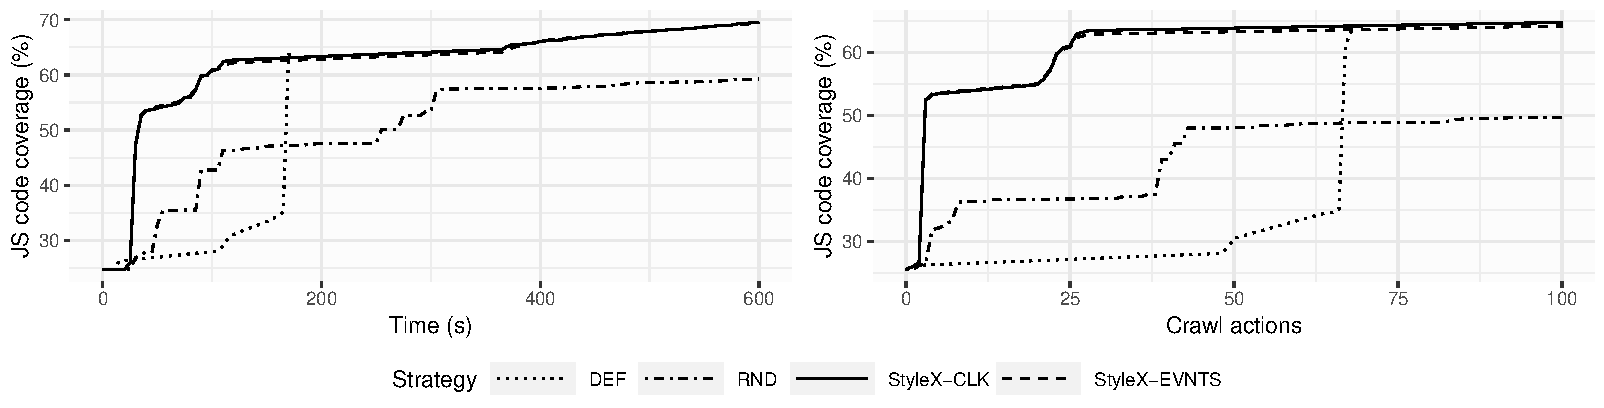
\includegraphics[width=\linewidth, trim={0 1.25cm 0 0}, clip]{figures/chess-coverage}
		\vspace{-6mm}
		\caption{p4wn (Chess)}
		\label{fig:coverage-chess}
	\end{subfigure}\\[8pt]
	\begin{subfigure}[b]{\linewidth}
		\centering
		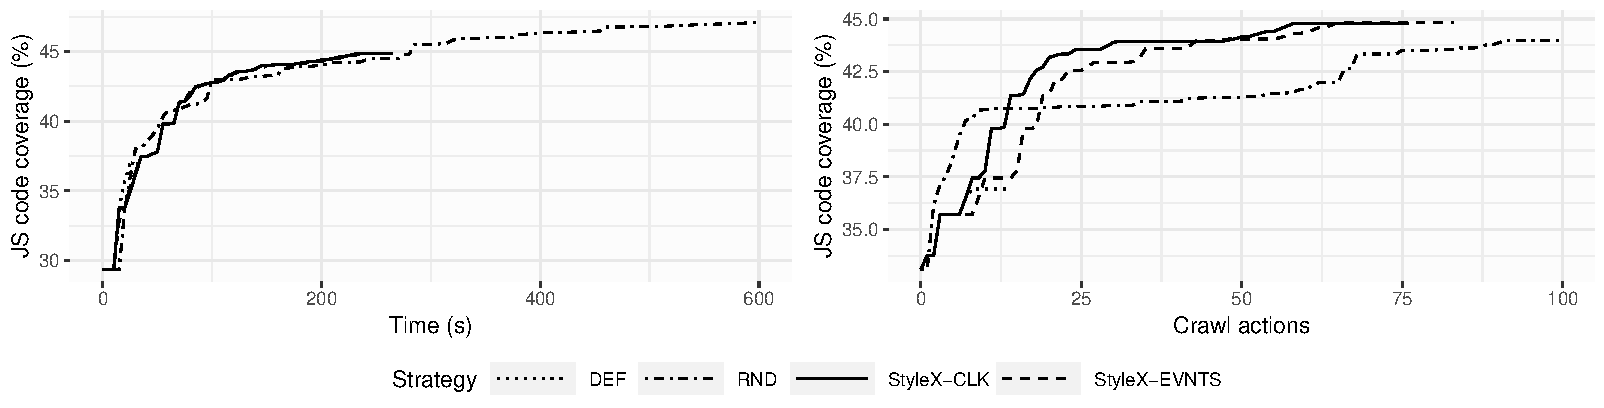
\includegraphics[width=\linewidth, trim={0 1.25cm 0 0}, clip]{figures/formbuilder-coverage}
		\vspace{-6mm}
		\caption{TacirFormBuilder}
		\label{fig:coverage-formbuilder}
	\end{subfigure}\\[8pt]
	\begin{subfigure}[b]{\linewidth}
		\centering
		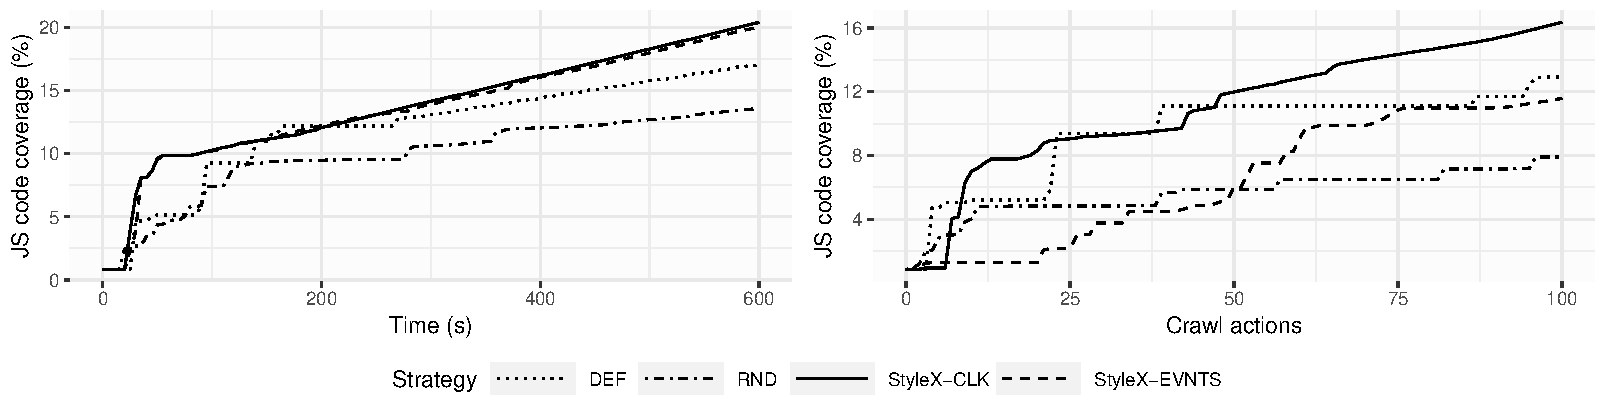
\includegraphics[width=\linewidth, trim={0 1.25cm 0 0}, clip]{figures/phormer-coverage}
		\vspace{-6mm}
		\caption{Phormer Photo Gallery}
		\label{fig:coverage-phormer}
	\end{subfigure}\\[8pt]
	\begin{subfigure}[b]{\linewidth}
		\centering
		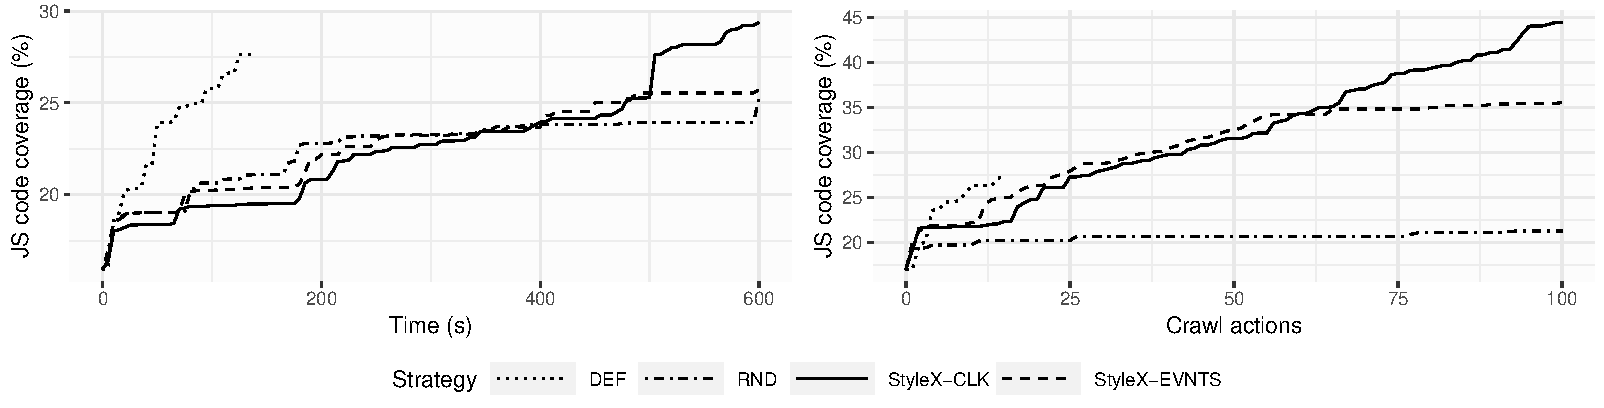
\includegraphics[width=\linewidth]{figures/calendar-coverage}
		\vspace{-4mm}
		\caption{Google Calendar}
		\label{fig:coverage-calendar}
	\end{subfigure}
	\caption{Coverage performance.}
	\label{fig:coverage-results}
\end{figure*}


\header{Measuring \js code coverage}
Measuring \js code coverage for dynamic web apps
is not a straightforward task.
For a crawler, the total number of lines of \js code
is typically unknown,
as \js code can be
injected dynamically at runtime
while exploring new states.
Previous work have disregarded the dynamically-injected code blocks 
when measuring code coverage~\cite{artzi2011framework};
however, we argue that they should be considered because they do occur
in reality,
especially for highly-dynamic web apps.
Therefore, 
we consider the largest set of \js code lines
that is found by any strategy during the crawl
(after all the crawl sessions are finished)
as the maximal set of lines of code that should be covered by the crawler
(i.e., a lower bound for the actual size of the \js codebase).
We then compute the code coverage as the percentage of code 
that is covered by each strategy over the size of the \js code in this maximal set.

We use the precise code coverage tool provided by
Chrome DevTools~\cite{chrome-dev-tools}.
Note that, since \js code can be obfuscated (i.e., shortened, concatenated into a single line), 
we report the coverage with respect to the number of characters covered,
as opposed to lines of code.
The \js size reported in \Cref{table:experimental-subjects} is calculated from this value.
This also includes the embedded and inline \js code blocks
(i.e., the code enclosed in the \code{<script>} tags and in the \html attributes concerning event listeners, e.g., \code{onmouseover}).

\subsubsection{Results}
We have illustrated the code coverage achieved
using different crawling strategies
in \Cref{fig:coverage-results},
for the constraints on time (left) and the number of crawl actions (right).

Observe in \Cref{fig:coverage-results} that, for all subjects,
the crawler finishes before the maximum time/number of crawl actions is reached
when only default clickables are considered (i.e., the \textit{DEF} strategy).
This essentially stresses the importance of considering elements 
other than default clickables when crawling,
also supporting the conclusions of an existing work~\cite{Behfarshad:2013:HiddenWeb}
on the importance of other element types for covering web app's state space.
Notice how including only clickables has led to achieving less final \js code coverage
compared to using our proposed technique.
Notwithstanding, we can see that in Google Calendar,
using default clickables yields more coverage earlier in crawling,
in contrast to other subjects.
This suggests that giving more priority to default clickables will not necessarily 
improve the crawling in terms of \js code coverage.

Also, observe in \Cref{fig:coverage-results} that 
supporting event types other than click 
did not necessarily help the approach 
in reaching significantly more \js code coverage.
This might be explained by the fact that there are more false positives 
in the prediction models for event types other than click,
i.e., the crawler might waste time firing actions on elements 
that do not actually have any events.
Nevertheless, it turns out that supporting these event types
can lead to achieving more code coverage
in shorter time and with fewer crawl actions in certain applications
(e.g., in Chess).

Within 10 minutes time limit, the maximum improvement in \js code coverage 
that \toolName can achieve over the \textit{DEF} strategy 
is 7.91\% (in TacirFormBuilder).
Compared to the \textit{RND} strategy,
the maximum improvement is 10.26\% (in Chess).
With click event only, 
\toolName outperforms the \textit{DEF} strategy by at most 7.91\% (in TacirFormBuilder)
and improves the \textit{RND} strategy by at most 10.22\% (in Chess).

Within 100 crawl actions,
the maximum improvement in \js code coverage that our approach 
can reach is by 8.16\%
compared to the \textit{DEF} strategy (in Calendar),
and by 14.51\% when compared to the \textit{RND} strategy (in Chess).
When considering the click event only,
the maximum improvement
shows up in Calendar:
\toolName can improve \js code coverage
by 17.02\% (compared to \textit{DEF}) and 23.19\% (compared to \textit{RND})
in Google Calendar.

Observe in \Cref{fig:coverage-results} that
\toolName achieves a much higher code coverage in the beginning of the crawling session
in Chess,
while the final code coverage value for both strategies might be close.
We noticed that in Chess the crawler with the \textit{DEF} strategy
keeps performing the same action across different states
by repeatedly clicking on one particular element,
while our approach can overcome this issue by ranking actionables.

In TacirFormBuilder, compared to the \textit{RND} strategy,
\toolName improves the \js code coverage marginally
when the number of actions is limited,
and underperforms when the time is limited.
This is because in this application,
on average, 46.31\% of the DOM nodes are actionable,
and the DOM is considerably small (\Cref{table:experimental-subjects}).
As a result, there is a high chance for a random strategy 
to achieve a high code coverage even in a short time.


